\documentclass[journal]{IEEEtran}
\IEEEoverridecommandlockouts

%%%%%%%%%%%%%%%%%%%%%%%%%%%%%%%%%%%%%%
%%%%%%%% PACCHETTI PRINCIPALI %%%%%%%%
%%%%%%%%%%%%%%%%%%%%%%%%%%%%%%%%%%%%%%
\usepackage{fancyhdr}
\usepackage{graphicx}
\usepackage[italian]{babel}
\usepackage[utf8]{inputenc}
\usepackage{color}
\usepackage{hyperref}
\usepackage{wrapfig}
\usepackage{array}
\usepackage{multirow}
\usepackage{adjustbox}
\usepackage{nccmath}
\usepackage{subfigure}
\usepackage{amsfonts,latexsym}
\usepackage{enumerate}
\usepackage{booktabs}
\usepackage{float}
\usepackage{threeparttable}
\usepackage{array,colortbl}
\usepackage{ifpdf}
\usepackage{rotating}
\usepackage{cite}
\usepackage{stfloats}
\usepackage{url}
\usepackage{listings}
\usepackage{soul}

%%%%%%%%%%%%%%%%%%%%%%%%%%%%%%%%%%%%
%%% CREA E SCRIVI ALCUNI COMANDI %%%
%%%%%%%%%%%%%%%%%%%%%%%%%%%%%%%%%%%%
\newcolumntype{P}[1]{>{\centering\arraybackslash}p{#1}}  %% Viene creato un nuovo tipo di colonna denominata P.

% correggere la sillabazione errata qui
\hyphenation{op-tical net-works semi-conduc-tor} %% Con questo comando si specifica come separare correttamente le sillabe nel caso in cui una parola si trovi in due diverse righe di testo

\graphicspath{ {./img/} }  %%Percorso dove si trovano le immagini, se è vuoto indica che le immagini sono all'interno della stessa cartella che contiene il file .tex


%%%%%%%%%%%%%%%%%%%%%%%%%%%%%%%%%%%%%%%%%%%%%%%%
%%% INTESTAZIONE DELLE PAGINE TIPO UNICAFAM %%%%
%%%%%%%%%%%%%%%%%%%%%%%%%%%%%%%%%%%%%%%%%%%%%%%%
\newcommand{\MYhead}{\smash{\scriptsize
\hfil\parbox[t][\height][t]{\textwidth}{\centering
\begin{picture}(0,0) \put(-30,-13){
\includegraphics[width=30mm]{logoUnisalento.jpg}} \end{picture} \hspace{6.4cm}
INGEGNERIA INFORMATICA \\
\hspace{5.2cm} DIPARTIMENTO DI INGEGNERIA DELL'INNOVAZIONE \hspace{3cm} \\
\underline{\hspace{ \textwidth}}}\hfil\hbox{}}}
\makeatletter

% normal pages
\def\ps@headings{%
\def\@oddhead{\MYhead}%
\def\@evenhead{\MYhead}}%

% title page
\def\ps@IEEEtitlepagestyle{%
\def\@oddhead{\MYhead}%
\def\@evenhead{\MYhead}}%
\makeatother

% make changes take effect
\pagestyle{headings}

% adjust as needed
\addtolength{\footskip}{0\baselineskip}
\addtolength{\textheight}{-1\baselineskip}

%define colors for code language
\definecolor{codegreen}{rgb}{0,0.7,0.3}
\definecolor{codegray}{rgb}{0,0,0}
\definecolor{codepurple}{rgb}{0.58,0,0.82}
\definecolor{backcolour}{rgb}{0.95,0.95,0.95}
\definecolor{keywordcolor}{rgb}{0.8,0.3,0}

\lstdefinestyle{mystyle}{
    backgroundcolor=\color{backcolour},   
    commentstyle=\color{codegreen},
    keywordstyle=\color{keywordcolor},
    numberstyle=\tiny\color{codegray},
    stringstyle=\color{codepurple},
    basicstyle=\ttfamily\footnotesize,
    breakatwhitespace=false,         
    breaklines=true,                 
    captionpos=b,                    
    keepspaces=true,                 
    numbers=left,                    
    numbersep=5pt,                  
    showspaces=false,                
    showstringspaces=false,
    showtabs=false,                  
    tabsize=4
}

\lstset{style=mystyle}



%%%%%%%%%%%%%%%%%%%%%%%%%%%%%%%%
%%%%% INIZIO DEL DOCUMENTO %%%%%
%%%%%%%%%%%%%%%%%%%%%%%%%%%%%%%%
\begin{document}



%%%%%%%%%%%%%%%%%%%%%%%%%%%%
%%% TITOLO DEL DOCUMENTO %%%
%%%%%%%%%%%%%%%%%%%%%%%%%%%%
\title{Pianificazione Automatica e \\sistemi di Supporto delle Decisioni}



%%%%%%%%%%%%%%%%%%%%%%%%%%
%%%%%%%%% AUTORE %%%%%%%%%
%%%%%%%%%%%%%%%%%%%%%%%%%%
\author{Matteo Aprile\\
				Professore: Giampaolo Ghiani, Enamuele Manni\\
        }
        
%scrive il titolo
\maketitle

%scrive l'indice
\tableofcontents
\underline{\hspace{ 80 mm }}



%%%%%%%%%%%%%%%%%%%%%%%%%%%%%
%%% SEZIONI DEL DOCUMENTO %%%
%%%%%%%%%%%%%%%%%%%%%%%%%%%%%
\section{Definizioni - 22/23.09.22}

Ci occuperemo di 2 tipi di scenari:
\begin{itemize}
	\item usare \hl{algoritmi a supporto delle decisioni}
	\item usare algoritmi che \hl{sostituiscono completamente l'uomo}
\end{itemize}


% Business Analytics
\subsection{Business Analytics}

Disciplina che utilizza dati, statistiche, modelli matematici per \hl{aiutare a prendere delle decisioni in base a dei dati}.

Possiamo racchiudere i suoi \hl{passaggi} in:
\begin{enumerate}
	\item \hl{descriptive analytics}: capire \textbf{cosa sia successo nel passato} tramite i dati disponibili
	\item \hl{predictive analytics}: cercare di \textbf{fare delle previsioni} in base ai dati già disponibili
	\item \hl{prescriptive analytics}: \textbf{creare un piano di azione} per poter massimizzare il KPI (Key Performance Indicator)
\end{enumerate}

\begin{figure}[H]
\centering
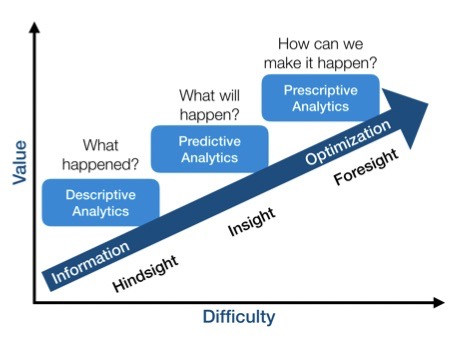
\includegraphics[scale=0.9]{businessAnalytics.jpeg}
\caption{Fasi della business analytics} 
\label{busana}
\end{figure}


% Decisioni
\subsection{Decisioni}

Rappresenta la \hl{scelta di un elemento tra più soluzioni} dopo aver ponderato le opzioni.

Possiamo avere più casi d'uso:
\begin{itemize}
	\item \hl{simplest case}: abbiamo \textbf{poche alternative} quindi una semplice scelta
	\item \hl{multple criteria}: abbiamo \textbf{più metri di paragone} delle performance, quindi si dovranno tenere in conto:
	
	\begin{itemize}
		\item \textbf{soluzioni migliori} di altre (dette di Pareto)
		\item \textbf{vincoli} dovuti dai clienti o da casi logistici da gestire (es: spedizioni)
		\item ottimizzazioni matematiche
		\item \textbf{conflitti tra i vincoli}
	\end{itemize}
	
	\item \hl{incertezze e rischi}: 
	
	\begin{itemize}
		\item \textbf{decisioni operative}: di \textbf{breve periodo}  \textbf{reversibili} e \textbf{limitate} a "n" persone del team
		
		\item \textbf{decisioni tattiche}: \textbf{coinvolge una parte dell'organizzazione} per un medio periodo
		
		\item \textbf{decisioni strategiche}: di \textbf{lungo periodo}  \textbf{non reversibili} e \textbf{coinvolgono denaro}
		
		\item \textbf{decisioni strutturate}: hanno una \textbf{procedura di risoluzione specifica}
		
		\item \textbf{decisioni non strutturate}: richiedono \textbf{creatività} ed \textbf{esperienza} in un  dato settore
	\end{itemize}
\end{itemize}

\begin{figure}[H]
\centering
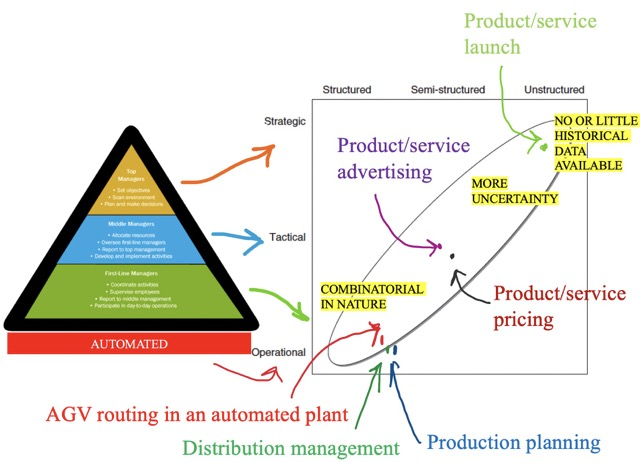
\includegraphics[scale=0.8]{dectax.jpeg}
\caption{Diagonale decisionale} 
\label{diadec}
\end{figure}


% Business Intelligence (BI)
\subsection{Business Intelligence (BI)}

Usato per indicare un \hl{sistema dedicato alla raccolta di dati e alla loro elaborazione} al fine di un reporting, infatti per "Inteligence" si intende investigazione.
Venivano \hl{usati su dati atomici} per avere delle conoscenze approfondite in un determinato business.


% Data visualization
\subsection{Data visualization}

Consiste nel \hl{prendere dati e plottare un grafico}, ma in realtà ora si ha una trattazione più metodologica, cioè se visualizzare in  modo statico o meno i dati.


% Decision Support Systems (DSS)
\subsection{Decision Support Systems (DSS)}

Si indicava un \hl{sistema computerizzato dotato di un sistema di "data managment"} per creare un modello di ottimizzazione, fornendo un feedback tramite un'interfaccia. Ora indica una varietà di sistemi per visualizzare i dati in larga misura o meno.


% Operations Research (OR)
\subsection{Operations Research (OR)}

\hl{Attivita organizzative per portare avanti un sistema logistico}. Per "research" si indica la ricerca delle operation per conseguire dei risultati, avremo come sottocategorie:
\begin{itemize}
	\item \textbf{ottimizzazione matematica}
	\item \textbf{queueing theory}: \textbf{studio matematico delle linee in attesa}  il limite è che funzionano solo con sistemi semplici e con richieste di servizio in ordine stocastico
	\item \textbf{simulazione}: per usarle è \textbf{necessario generare dei numeri randomici}  \textbf{quindi  inconveniente} (bisogna fare un analisi statistica dei risultati dalle quali si farà una \textbf{stima} 
	\item \textbf{game theory}: decisioni con \textbf{più players}
\end{itemize}


% Agents
\subsection{Agents}

È un \hl{sistema che si muove in un environment} (ambiente), ha dei \hl{sensori} tramite i quali percepisce alcuni aspetti del mondo che lo circonda quindi si crea una \hl{rappresentazione del mondo circostante} che può vedere. È capace di \hl{influenzare l'ambiente tramite degli attuatori} come ruote o braccia (intendiamo anche agenti software).

Possiamo classificarli come:
\begin{itemize}
	\item \hl{agenti autonomi}: se è concepito in modo tale che \textbf{tramite un'istruzione sintetica raggiunge un goal sviluppando le azioni per raggiungerlo}  In realtà può anche non essere una sequenza di azioni dato che \textbf{potrebbero esserci degli imprevisti}
	\item \hl{agenti intelligenti}: se
	\item \textbf{impara dall'esperienza}
	\item crea una \textbf{rappresentazione dell'ambiente} che lo circonda e \textbf{ci ragiona sopra} per un possibile risultato delle proprie azioni
	\item \textbf{si adatta ad un ambiente mutevole}
\end{itemize}

\begin{figure}[H]
\centering
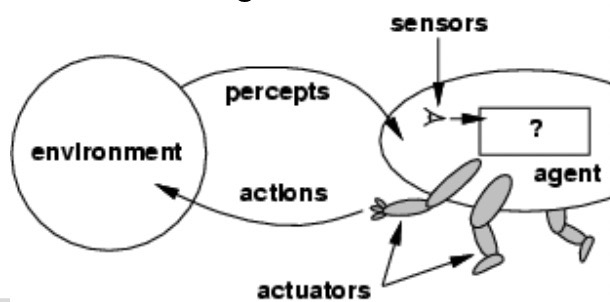
\includegraphics[scale=0.6]{agents.jpeg}
\caption{Schematizzazione di un agente e sue caratteristiche} 
\label{agente}
\end{figure}


% Artificial Intelligence (AI)
\subsection{Artificial Intelligence (AI)}

Comprende tante sottodiscipline:
\begin{itemize}
	\item \hl{automated reasoning}: legato alla \textbf{rappresentazione del mondo} e \textbf{come raggionare su di essa} ma anche calcolandone le probabilità
	\item \hl{automated planning}: usato in ambienti industriali
	\item \hl{automated learning}
	\item \hl{natural language processing}: \textbf{sviluppare agenti software} per fare sintesi di testi, scrivere automaticamente articoli, chat bot, ecc 
	\item \hl{perception}: visione artificiale
	\item \hl{manipuliation}: avere un \textbf{agente che può modificare l'agente} circostante
\end{itemize}


% Machine Learning (ML)
\subsection{Machine Learning (ML)}

Consiste nell'\hl{apprendimento automatico} e quindi lo sviluppo degli \hl{agenti che apprendo tramite la loro esperienza pregressa}. Ci sarà allora una fase di \hl{training}.
Una delle possibili \hl{architetture che permette di farlo sono le Neural Networks} prima avevano solo 2/3 neuroni, ora ne hanno vari strati il che fornisce delle prestazioni impressionanti


% Deep Leaning
\subsection{Deep Leaning}

Si basa sull'\hl{apprendimento automatico} con reti neurale tramite un gran numero di strati di neuroni.


% Data Mining (DM)
\subsection{Data Mining (DM)}

Usare metodi di Machine Learning per \hl{estrarre manualmente dei pattern dai dati}, cioè una \hl{regolarità o un trend}. È quindi la parte nobile del knowledge discovery in db, dato che i dati sono in genere disponibili su db o da altre piattaforme.

La \hl{sequenza} nella quale interviene è:
\begin{enumerate}
	\item \textbf{prendere} i dati
	\item trovare i vari \textbf{target}
	\item \textbf{preprocessare} i dati
	\item trasformare i dati tramite il \textbf{data mining}
	\item trovare dei \textbf{patterns} (dopo il data mining)
\end{enumerate}



































\section{28.09.22}

RIEPILOGO DI CONCETTI DI BASE DEI DB RELAZIONALI:

cap 1: database
1. definizioni di base:
dato: insieme di fatti conosciuti registrati con un significato. Sono detti dati grezzo visto che si suppone che andrò a elaborarlo, questo dato sarà poi archiviato, sarà un fatto conosciuto cioè degli eventi con un significato per un dato tipologia di utenti ed e1 conosciuto dato che c'e1 una sorgente che produce i dati con una cerca velocità.

database: raccolta di dati altamente organizzati intercorrelati e strutturati. e1 una struttura con dei collegamenti strutturati tra i dati

dbms: data base managment system: insieme di programmi per accedere ai dati e farci delle operazioni di 4 tipi: creazione, recupero, aggiornamento e cancellazione, ciclo CRUD.

esistono molti tipi di db i primi erano solo numerici o testuali, ora ci sno nquelli multimediali, GIS Geographic Information Systems, data warehouses

opportuno vedere dei concetti di base. i dati hanno un ciclo di vita, il piu1 semplic è:
acquisizione (scattered data) -> aggragazione (integrated data) -> alisi (knowledge) -> finisce in un apllicaizone che genera dei log data che sarannp poi acquisiti come scattered data

da u punto di vista computazionele queste fasi si devono prendere in un altro modo:
1. storage dei data
2. formattazione e pulizia
3. capire cosa i dati ci dicono 
3.? se non mi bastano i dati che ho posso integrare dei dati 

definizioni:
database: collezione di dati collegati tra loro

mini-world: parte del mondo real ai quali si riferiscjno i dati presi. per creare un database vado a limitare la modellazione in un numero n di concetti

dbms: sistema che afacilita mantenimento e gestiondel db

database system: insieme di dbms con i dati


quando si ha un db abbiamo 3 livelli da considerare
fisico (dove sono salvati
logico: come sono collegati tra loro
vista: rappresentazione che sarà diversa per ogni tipo di utente


da un punto di vista architetturale da un aparte ho gli utenti a dall'altra i dati e i metadati (che descrivono i dati). avrò bisognodi un software per eseguire le query 

un dbms offre:
di db mi consente di fare più del semplice slvataggio:
definire modelli dati
manipolarli
processarli e condividerli

per interagire coi db possono esere tramite:
query: accede a parti differenti di dati e formula una richiesta
transazioni:legge dei dati ed aggiorna alcuni valori e li salva nel db


nei nostri mini-world avremo bisogno di identificare delle entità cioè i concetti di base che rappresentano una parte delle cose che inseriremo nel db relaizonele il resto sta nel connettere tra loro le entità, dette relazioni (relationships) (ER) le tabelle che ne derivano sono dette relation. tutto cio deve derivare dai requisiti e non dal'esperienza personale.

le entità diventano delle tabelle dove inseirisco i dati che ho a disposizione che saranno divise per righe (record) e colonne (attributi) i singoli elementi sono i dati grezzi

catalogo dei dbms ci sono i vincoli creati da un software specifico, i ltipo dei dati e la relaizone di appartenenza degli attrbuti

concetto fondamentale: astrazione:
ho dei dati e collegamenti tra varie entità e dei modi per salvrli. dobbiamo separare le cose per disporre di un modello senza che esso si occupi di come salvare i dati

modello concettuale:

modello fisico: definiziaone dei tipi dato e dove sono conservati

controllo della concorrenza: garantire ceh tuttle le transazioni sono correttamente eseguite
recovery: se la transazione è stat eseguita e1 stata recorded nel database




cap 2: 


data model: insieme di concetti che descrivon ola struttura di un db, le operaizoni e i vincoli applicati al db

data model structure e constraints: abbiamo dei costrutti che definiscono come collegare gli elemtni definiti da: entità, record e tabella
i vincoli devono essere sempre rispettati e bloccanti

data model operation: di base (CRUD) o definite dall'utente

modello dato di tipo concettuale: di alto livello e semantico

mkodello fisico: definisce come i dati sono salvati, basso livello

modello tipo implementativo: usati nel dbms 

modello implementation: provide concepts taht fall between the above two

modello autodescrivente: basati su XML 



3 definizioni fondamentali:
database schema: descrizione del database in termini di sctuttura tipo dati e vincoli

schema diagram: visione rappresenzativa del db schema

schema construct: insieme tra schema ...


figura 2.1 schema diagram

database state: smapschot in istante t del db, si devfinisce quidni ai suoi contenuti

valid state: si definisce funzionante se il suo contenuto soddifa i vincoli per quello schema

nota che:
schema può esere detto intensio
state può essere detto extension


abbiamo 3 livelli di schema:
interno (fisico): come i dati devono essere salvati e come posso accederci
concettuale
esterno: per descrivere le view dell'utente


per passare d aun o schema ad un ator ho bisogno di un mapping per capire a cosa corrsponde un elemento. avremo che:

logic data independence: se voglio cambiare lo schema concettuale senxa cambiar equello fisico

physiccal; devo cambiare lo schema sifico senza cambiare quello concettuale



qundo ho un data manipulation language dml posson usarlo inautonomia o inserirlo in un orogramma facendop tramite:
embedded approsh (tramite java, c ...)
procedure call approach
db programming language approach
scripting languages


definizione
data dictioraty: insime dove salvo sia lo schema che altre info 



abbiamo più tipologi e di dbms:
centralized: dfove abbiamo tutta l'eleborazioe su un unico nodo

2-tier: sistpecializza in termini di server per ogni blocco di funzionalità che devo offrire

cliets: per far accedere gli utenti

dbms server: per esegjuire query e transazioni tramite API 

three-tier: abiamo 3 livelli: ...






%%%%%%%%%%%%%%%%%%%%%%%%%%
%%%%%% BIBLIOGRAFIA %%%%%%
%%%%%%%%%%%%%%%%%%%%%%%%%%
\begin{thebibliography}{1}

\bibitem{nome_bibliografia}
	\url{https://en.wikibooks.org/wiki/LaTeX/Hyperlinks}
\end{thebibliography}


\end{document}
%%%%%%%%%%%%%%%%%%%%%%%%%%%%%%%%
%%%%%% FINE DEL DOCUMENTO %%%%%%
%%%%%%%%%%%%%%%%%%%%%%%%%%%%%%%%




